
%%-----------------Chapter 7---------------------------
\chapter{Systems Biology Research with Hybrid Automata}\label{chap:research}

While directly solving the equation $Sv = 0$ to receive the set of bases $B = \{ b_1, b_2, ..., b_n \}$ is sufficient to satisfy the constraints of the framework and build a phenotypically-sound microbial model, this naive formulation is not optimized for the experimentation and analysis tasks demanded by research practitioners. As discussed in Chapter \ref{chap:sys}, there are a number of methods from the systems biology literature that decompose the steady-state flux space into a set of convex bases. These methods are preferred because they offer phenotypically-relevant context that allows the researcher to interpret the functional significance of the individual bases within the broader metabolic network. When building a framework for experimentation and analysis with the ultimate goal of furthering explainability of metabolic processes, such additional context is invaluable to both the model itself (insofar as it offers additional properties that can be formalized, traced, and verified) and to the researcher (by providing a helpful elucidation of the biological significance of otherwise opaque formalisms). Thus, the modelling framework with hybrid automata can be enhanced by replacing the set of bases $B = \{ b_1, b_2, ..., b_n \}$ with the convex bases rendered by one of the systems biology approaches for decomposing the flux cone. The theoretical implications as well as practical concerns raised when employing these approaches is detailed further below. A brief discussion of the advanced analytical capability provided by the enhanced model, with details of how it could be harnessed in a research pipeline, is also included.

As a reference point, the general form of an organism automaton (as discussed in Chapter \ref{chap:model}) is given below. Modifications to this form, brought on by the replacement of the $B = b_1, b_2, ..., b_n$ vectors, will be presented in the following sections. The nondeterministic form is essential to the generality of the model. The distinct benefits (as well as potential drawbacks) of replacing the nondeterminism with a defined control mechanism will be a key point of discussion in a section to follow. As a side note, the growth mechanism given is the same as Chiu's formulation, but it need not necessarily be. A more straightforward growth mechanism would also suffice without loss of generality. 

 \begin{figure}[H]
\centering
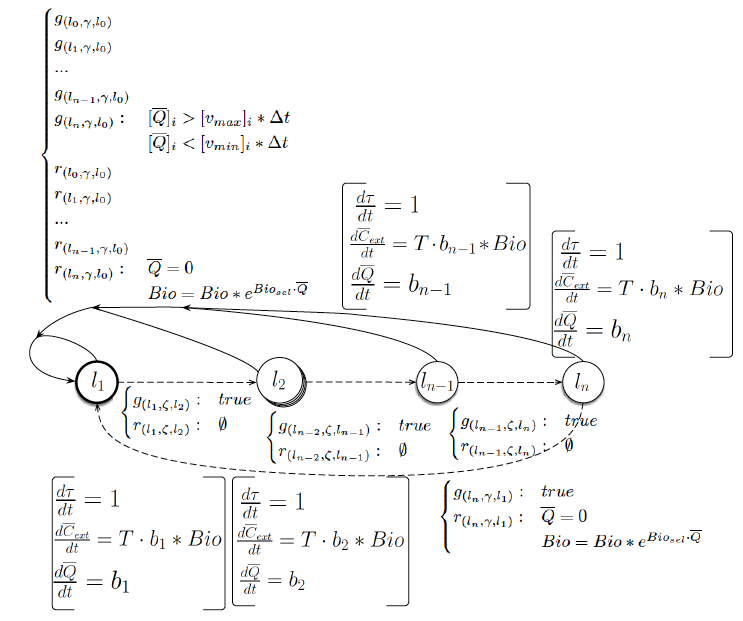
\includegraphics[width=1.0\textwidth]{figures/regulatory1.png}
\caption{General form of a microbe automaton using naive bases}
\label{Organism2Automata}
\end{figure}


\section{Extreme Pathways to Regulatory Mechanisms}

% Using techniques from extreme pathways analysis, we can isolate the regulatory mechanisms and sub-networks responsible for emergent metabolite production and identify the intervals in which they are active. We can then find the environmental shifts that induce emergent behavior, retrace the sequence of shifts together with the corresponding regulatory modes, and discover the parameters (of both the medium and the organisms) under which emergent metabolite production is maximized.

\subsection{Singular Value Decomposition and Eigenpathways}


 As discussed in Chapter \ref{chap:sys}, the extreme pathways are a set of convex bases that fully characterize the phenotypically viable solution space. However, without a corresponding kinetic model, the extreme pathways alone cannot be used to directly elucidate the underlying regulatory mechanisms that give rise to metabolic processes. Singular value decomposition can be applied to the matrix of extreme pathways (or \textit{expas}), wherein the left singular vectors of the SVD are the \textit{eigenpathways} of the metabolic network. The eigenpathways have been shown to characterize the physiologically relevant metabolic states that would otherwise be computed with a detailed kinetic model. Furthermore, in the case of the red blood cell metabolism, the first five (in order of significance) eigenpathways out of a total of 23 characterize the relevant regulatory mechanisms that underlie shifts in metabolic behavior. Thus, the use of eigenpathways instead of the raw expas implicitly reduces the dimensionality of the viable flux space. In the case of the red blood cell metabolism, only five degrees of freedom are needed to characterize 91\% of the relevant fluxes within the flux cone.
 
 
 % underlying regulatory 

% https://pubmed.ncbi.nlm.nih.gov/14575652/
% https://pubmed.ncbi.nlm.nih.gov/16533395/
% https://journals.plos.org/plosone/article?id=10.1371/journal.pone.0210539



%Reconstruction of cell-scale metabolic networks is now possible. A description of allowable metabolic network functions can be obtained using extreme pathways, which are the convex basis vectors of the solution space containing all steady state flux distributions. However, only a portion of these allowable network functions are physiologically possible due to kinetic and regulatory constraints. Methods are now needed that enable us to take a defined metabolic network and deduce candidate regulatory structures that control the selection of these physiologically relevant states. One such approach is the singular value decomposition (SVD) of extreme pathway matrices (P), which allows for the characterization of steady state solution spaces. Eigenpathways, which are the left singular vectors from the SVD of P, can be described and categorized by their biochemical function. SVD of P for the human red blood cell showed that the first five eigenpathways, out of a total of 23, effectively characterize all the relevant physiological states of red blood cell metabolism calculated with a detailed kinetic model. Thus, with five degrees of freedom the magnitude and nature of the regulatory needs are defined. Additionally, the dominant features of these first five eigenpathways described key metabolic splits that are indeed regulated in the human red blood cell. The extreme pathway matrix is derived directly from network topology and only knowledge of Vmax values is needed to reach these conclusions. Thus, we have implemented a network-based analysis of regulation that complements the study of individual regulatory events. This topological approach may provide candidate regulatory structures for metabolic networks with known stoichiometry but poorly characterized regulation.


For an automata model of a microbe, the set of bases $B = \{ b_1, b_2, ..., b_n \}$ can be replaced by the set of eigenpathways $E = \{ e_1, e_2, ..., e_m \}$ rendered by the SVD of the expas of $S$, without loss of generality. Furthermore, $E$ can be restricted to the significant subset $E_k = \{ e_1, e_2, ..., e_k \}, k \leq m$, such that the relevant flux space is still effectively characterized but the degrees of freedom of the model (and locations in the automaton) are greatly reduced. This renders the model more compact and hence computationally efficient while also adding additional interperability for the researcher designing and running experiments.

 \begin{figure}[H]
\centering
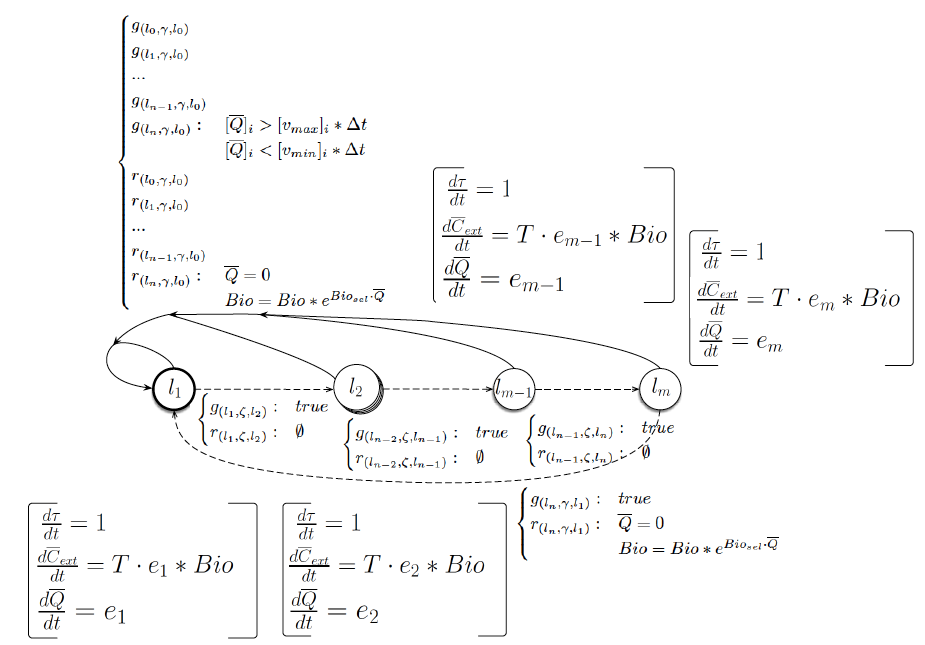
\includegraphics[width=1.0\textwidth]{figures/regulatory3.png}
\caption{Microbe automaton as parameterized by the eigenpathways}
\label{Organism2Automata}
\end{figure}

 \begin{figure}[H]
\centering
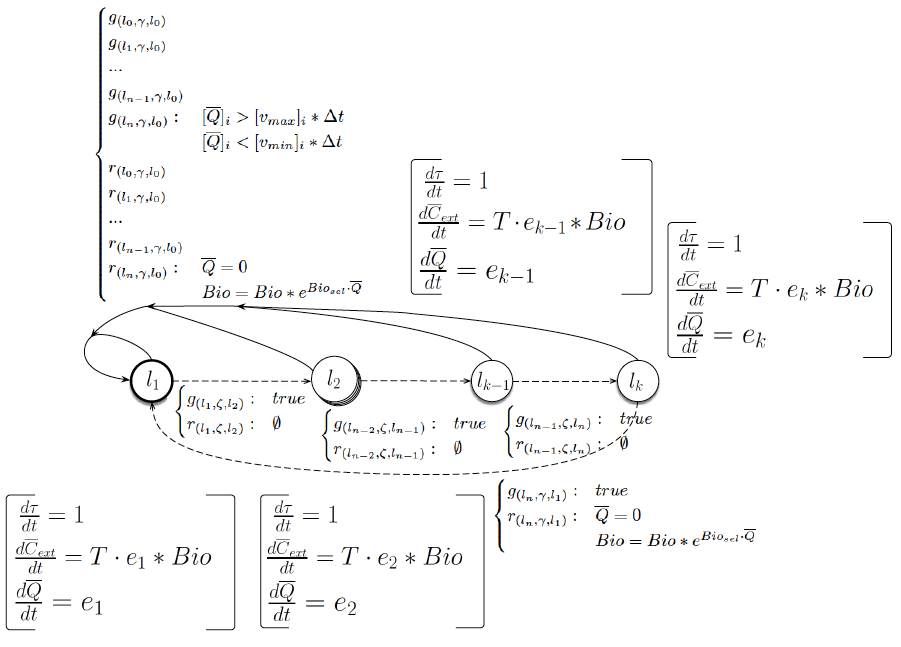
\includegraphics[width=1.0\textwidth]{figures/regulatory2.png}
\caption{Microbe automaton as parameterized by $E_k$. Generally, $k << m$, rendering the model significantly more computationally efficient.}
\label{Organism2Automata}
\end{figure}

% question: in above, is n=m??

% this is a model using the naive bases

% becomes model using eigenpathways instead of b1... bn

% when restricting eigenpathways to significant pathways, show how automata changes

% maybe include experimental results showing how most trajectories can still be taken
% but time to explore is greatly reduced?

\subsection{Nondeterministic Regulatory Dynamics}

With the parameterization $E_k = \{ e_1, e_2, ..., e_k \}$ that directly relates locations in the automaton to regulatory modes, more robust experiments can be run than the naive parameterization alone supports. Experiments of the following nature can be posed and answered:

\begin{enumerate}
    \item Do the trajectories that lead to failure under some safety analysis scenario always include or exclude a specific regulatory mode?
    \item Is emergent metabolism (in a co-culture automata) dependent on some regulatory mode in one (or both) of the microbes being reached?
    \item Is a specific sequence of regulatory shifts a necessary precursor to some metabolite to be produced?
    \item Will a specific regulatory shift always result in some metabolite being produced?
\end{enumerate}

Answering these questions involves exhaustive exploration of the solution space, using the nondeterminism present in the model to guarantee the realization of all valid trajectories. The newly established relationship between locations and regulatory modes allows the regulatory shifts taken to be embedded in the trajectory itself, along with the concentrations of metabolites. The regulatory mode represented by location $l_i$ is $r_i$.

Within each forward ``run", a sequence of regulatory shifts is realized as the locations are traversed. Since the time spent in each location corresponds to the net time in a regulatory mode, only consider locations that have $\Delta t_i > 0, 1 \leq i \leq k$. Thus, upon the transition $l_n \Rightarrow l_1$, the set $R = \{ r_i \; | \; l_i \in L, \; \Delta t_i > 0, \; 1 \leq i \leq k \}$ represents the regulatory modes entered while realizing some flux vector $v$. This set of regulatory modes is implicitly ordered as the forward transition topology forces an ordering onto the locations $l_i$. Thus, a sequence of forward ``runs" realizing the trajectory $\mathbb{D}(\overline{V} = [v_1, v_2, ..., v_n])$ induces a sequence of sets $[R_1, R_2, ..., R_n]$. As the sets themselves are implicitly ordered, this sequence can be ``flattened" into a one-dimensional vector of regulatory modes $\overline{R} = [r_1, r_2, ...]$. This is the sequence of regulatory shifts taken when realizing $\mathbb{D}(\overline{V})$.

Thus, when exploring the solution space by enumerating all $\{ \mathbb{D}(\overline{V})\}$, the subset of $\{ \mathbb{D}(\overline{V})\}$ that satisfies some reachability condition (emergent metabolite production, failed safety analysis property) can have queries regarding regulatory shifts evaluated over $\{ \overline{R} \}$.

The above necessitates the development of a formalization that unifies reachability queries in the continuous space with properties to evaluate over the location-space induced by all satisfiable trajectories.

%$\overline{Q} = v \Delta t$



%% what can be gained from nondeterministic formulation BUT locations = regulatory modes

% will emergent metabolite be produced in one location only?

\subsection{Formalizing Regulatory Queries}

Continuous property satisfied $\Rightarrow$ Query over sequence of locations

% and querying the model for specific regulatory information

\subsection{From Optimal Control to Regulatory Mechanisms}

The newly established correspondence between locations and regulatory mechanisms makes the optimal control problem on organism automata significantly more symbolically meaningful. When locations come to represent regulatory modes, solving for the control functions that deliver a near-optimal trajectory with respect to some objective translates into finding the environmental conditions that trigger a regulatory shift. This presents a tremendous leap forward in the analytical ability that the automata framework provides for analyzing and explaining metabolic behavior. When using the naive bases, the optimal control problem could be formulated and solved on the automaton, allowing the researcher to observe the environmental shifts underlying emergent metabolic capacity, but provided no additional interperability nor explainability over the dFBA approach. The transition behavior was a ``black box" from the perspective of the researcher. Incorporating eigenpathways (and hence regulatory mechanisms) into the framework allows the unification of steady-state metabolic simulation with detailed analysis of regulatory mechanisms \textit{without} requiring any sort of kinetic model that the existing approaches integrating regulation with dFBA rely upon. With this capability in mind, the environmental conditions along with the relevant regulatory shifts that trigger emergent behavior in co-culture models can be studied and isolated. Furthermore, complex metabolic engineering scenarios (with one or more microbes present) can be formulated wherein the regulatory shifts observed can be compared to a well-studied reference model to verify the soundness of the \textit{in silico} behavior. Like the other components of this modelling framework, knowledge of the stoichometry is all that is needed to build and verify microbial models, with no assumptions made about the kinetic mechanisms underlying the metabolic behavior.

The OC problem is also computationally simpler to solve when parameterizing the model with eigenpathways -- the reduction in degrees of freedom results in $k$ total locations instead of the original $m$/$n$. Hence, only $G_{h}(\overline{C}_{ext})$, $1 \leq h \leq k$ deterministic control functions must be found.

\begin{figure}[H]
\centering
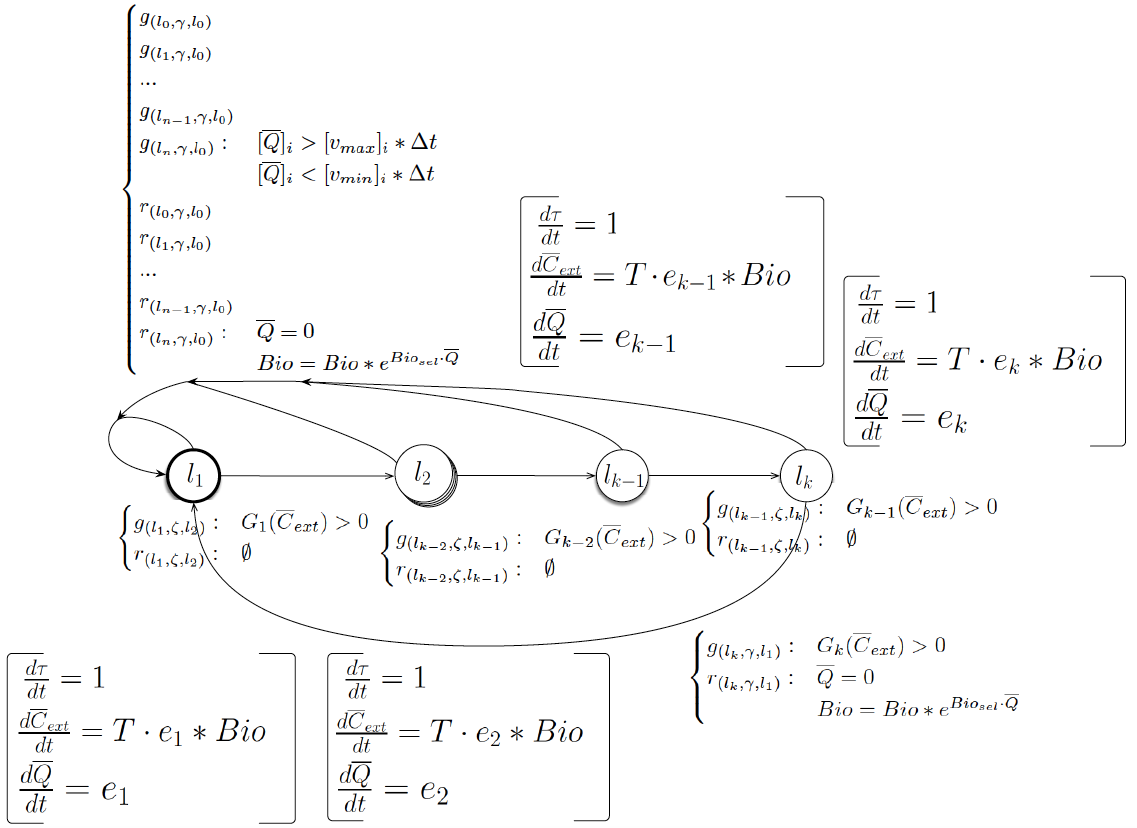
\includegraphics[width=1.0\textwidth]{figures/regulation-with-control.png}
\caption{Microbe automaton with $E_k$ parameterization and deterministic control functions.}
\label{Organism2Automata}
\end{figure}


Before considering this a realistic model of regulatory shifts, a question must be raised regarding the transition topology of this model versus the traditional model of regulatory behavior. Specifically, the most general model of regulation allows for transitions between each pair of regulatory modes as in the diagram that follows:

\begin{figure}[H]
\centering
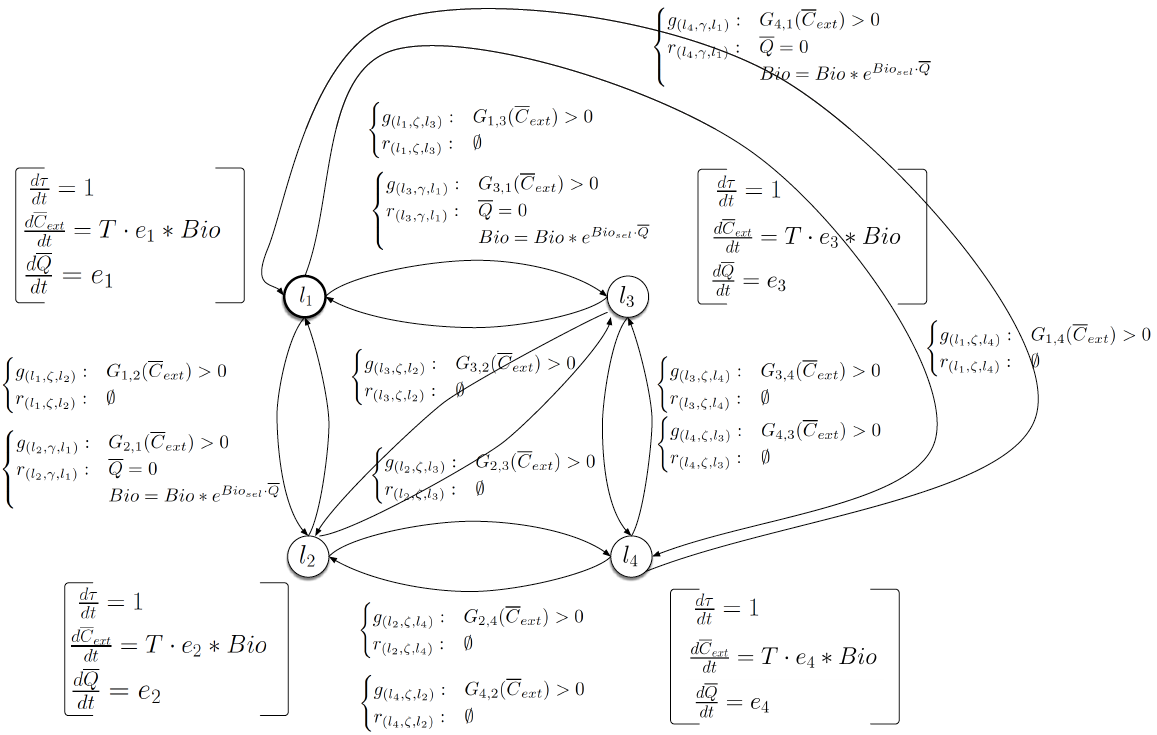
\includegraphics[width=1.0\textwidth]{figures/regulatory-full-4-loc.png}
\caption{Automaton representing cellular regulation as generally understood. Each regulatory mode can transition to any other regulatory mode. $k=4$ has been chosen but $k$ is arbitrary. Transitions to $l_1$ driven by $[\overline{Q}]_i > [v_{max}]_i * \Delta t$ and  $[\overline{Q}]_i < [v_{min}]_i * \Delta t$ have been omitted for clarity but would be present in the model.}
\label{Organism2Automata}
\end{figure}

A similar model is featured in (paper) as part of their regulatory-kinetic hybrid automaton model of cellular metabolism. It is not immediately clear if the flux-based model (with eigenpathways) that features only forward transitions between locations $l_1, ..., l_k$ fully encapsulates the same range of behaviors. For this model to suffice, a bisimulation must be drawn between the two.

In the case of the model with only forward transitions along $l_1, l_2, ..., l_k$, the control mechanism for some location $l_i$ must be established that the transition is triggered whenever another location is desired, regardless of the proper originating location for such a transition in the fully connected automaton. Consider the case where $k = 4$. If the current location is $l_3$ and the transition activated is $l_3 \rightarrow l_2$, in the fully connected automaton, that transition will be triggered directly by the control mechanism $G_{3,2}(\overline{C}_{ext})$. However, the model with only forward transitions does not have a direct transition between location $l_3$ and $l_2$ and hence no control mechanism can properly be defined over it. The path $l_3 \rightarrow l_4 \rightarrow l_1 \rightarrow l_2$ instead must be taken and the control mechanism $G_{3,2}(\overline{C}_{ext})$ that signifies the environmental conditions inducing the regulatory shift must govern all three of those transitions. Furthermore, the elapsed time in $l_4$ and $l_1$ must be zero - a regulatory mode $r_i$ is only considered enabled if $\Delta t_i > 0$. To represent a regulatory shift from $r_3$ directly to $r_2$, the transitions $l_4 \rightarrow l_1$ and $l_1 \rightarrow l_2$ must fire instantaneously upon entering the originating state.

%% reformulate below to use union of sets instead of and
% each G(.) is a function over the continuous space (X -> R)  ... want to define guards as subset of space
% where some condition holds true
% guards are combined by unioning these individual subsets of the space

To solve the above dilemma, control functions along the forward transitions (counting $l_4$ to $l_1$ at the end of a ``run" as a forward transition) should be defined as follows:
\begin{equation*}
    \begin{split}
        G_{1}(\overline{C}_{ext}) = \; & G_{1,2}(\overline{C}_{ext}) > 0 \; || \; G_{1,3}(\overline{C}_{ext}) > 0 \; || \; G_{1,4}(\overline{C}_{ext}) > 0 \; || \; \\
         & G_{2,3}(\overline{C}_{ext}) > 0 \; || \; G_{2,4}(\overline{C}_{ext}) > 0 \; || \; \\
         & G_{3,2}(\overline{C}_{ext}) > 0 \; || \; G_{3,4}(\overline{C}_{ext}) > 0 \; || \; \\
         & G_{4,2}(\overline{C}_{ext}) > 0 \; || \; G_{4,3}(\overline{C}_{ext}) > 0 \\
         %%%%%%%%%%%%%%%%%%%%%%%%%%%%%%%%%%%%%%%
         G_{2}(\overline{C}_{ext}) = \; & G_{2,1}(\overline{C}_{ext}) > 0 \; || \; G_{2,3}(\overline{C}_{ext}) > 0 \; || \; G_{2,4}(\overline{C}_{ext}) > 0 \; || \; \\
         & G_{1,3}(\overline{C}_{ext}) > 0 \; || \; G_{1,4}(\overline{C}_{ext}) > 0 \; || \; \\
         & G_{3,1}(\overline{C}_{ext}) > 0 \; || \; G_{3,4}(\overline{C}_{ext}) > 0 \; || \; \\
         & G_{4,1}(\overline{C}_{ext}) > 0 \; || \; G_{4,3}(\overline{C}_{ext}) > 0 \\
         %%%%%%%%%%%%%%%%%%%%%%%%%%%%%%%%%%%%%%%
         G_{3}(\overline{C}_{ext}) = \; & G_{3,1}(\overline{C}_{ext}) > 0 \; || \; G_{3,2}(\overline{C}_{ext}) > 0 \; || \; G_{3,4}(\overline{C}_{ext}) > 0 \; || \; \\
         & G_{1,2}(\overline{C}_{ext}) > 0 \; || \; G_{1,4}(\overline{C}_{ext}) > 0 \; || \; \\
         & G_{2,1}(\overline{C}_{ext}) > 0 \; || \; G_{2,4}(\overline{C}_{ext}) > 0 \; || \; \\
         & G_{4,1}(\overline{C}_{ext}) > 0 \; || \; G_{4,3}(\overline{C}_{ext}) > 0 \\
         %%%%%%%%%%%%%%%%%%%%%%%%%%%%%%%%%%%%%%%
         G_{4}(\overline{C}_{ext}) = \; & G_{4,1}(\overline{C}_{ext}) > 0 \; || \; G_{4,2}(\overline{C}_{ext}) > 0 \; || \; G_{4,3}(\overline{C}_{ext}) > 0 \; || \; \\
         & G_{1,2}(\overline{C}_{ext}) > 0 \; || \; G_{1,3}(\overline{C}_{ext}) > 0 \; || \; \\
         & G_{2,1}(\overline{C}_{ext}) > 0 \; || \; G_{2,3}(\overline{C}_{ext}) > 0 \; || \; \\
         & G_{3,1}(\overline{C}_{ext}) > 0 \; || \; G_{3,2}(\overline{C}_{ext}) > 0 \\
    \end{split}
\end{equation*}

More generally, this formulation can be written for some automaton with $k$ indeterminate as:
\[
    \large
    G_{i}(\overline{C}_{ext}) = \bigcup^k_{\substack{n,m=1 \\  n \neq m \\ m \neq i}} G_{n,m}(\overline{C}_{ext}) > 0
\]

It must be shown that, given the control functions as defined above, some environmental trigger for a regulatory shift in the fully-connected automaton will induce the same regulatory behavior in the forward-connected automaton. Showing full regulatory sequence equivalence is not necessary, as behavioral equivalence upon the same set of environmental triggers will invariably lead to regulatory sequence equivalence between the two automata.

For the fully-connected automaton, $G_{3,2}(\overline{C}_{ext}) > 0$ in $l_3$ will directly fire a transition from $l_3$ to $l_2$ representing the regulatory shift from $r_3$ to $r_2$. No further elucidation is necessary in this case.

However, in the forward-connected automaton, $G_{3,2}(\overline{C}_{ext}) > 0$ in $l_3$ will trigger $G_{3}(\overline{C}_{ext})$ firing $l_3 \rightarrow l_4$. Upon entering $l_4$, the relation $G_{3,2}(\overline{C}_{ext}) > 0$ still holds and triggers $G_{4}(\overline{C}_{ext})$ firing $l_4 \rightarrow l_1$. Again, $G_{3,2}(\overline{C}_{ext}) > 0$ is still valid upon entering $l_1$ and triggers $G_{1}(\overline{C}_{ext})$, firing $l_1 \rightarrow l_2$. Finally, upon reaching $l_2$, $G_{3,2}(\overline{C}_{ext}) > 0$ holds but is not a component element of $G_{2}(\overline{C}_{ext})$, leading the system to stay in $l_2$ for some $\Delta t_2 > 0$. Since the elapsed time in both $l_4$ and $l_1$ is $0$, the sub-sequence of regulatory shifts induced is simply $r_3 \rightarrow r_2$.


%% biomass and vector should NOT be reset when taking regulatory transitions
%% big difference from nondeterministic representation



\section{From Genome-Scale Models to Hybrid Automata}

Genome-scale models are the state-of-the-art in modern systems biology research, providing the ability to study real-world organisms \textit{in silico} by providing a tremendously detailed description of the internal stoichiometry. High-definition genome sequencing techniques are employed to build accurate stoichiometric models on the order of tens of thousands of individual reactions. However, a number of computational issues must be rectified before genome-scale models can be fully integrated into the hybrid automata framework. The tabular approach for finding extreme pathways quickly becomes computationally intractable on a system of thousands of linear equations. Thus, an alternative method for computing extreme pathways should be devised such that the structure of the flux cone is preserved while the convex bases themselves are computable in polynomial time.

\subsection{Sampling the Flux Space}

Paullson and co. have devised a method to compute extreme pathways by repeated statistical sampling of the flux space.

\subsection{A Genome-Scale Analytical Pipeline}

Putting the previous sections together allows the full pipeline for experimentation on genome-scale models to be formalized.

\begin{figure}[H]
\centering
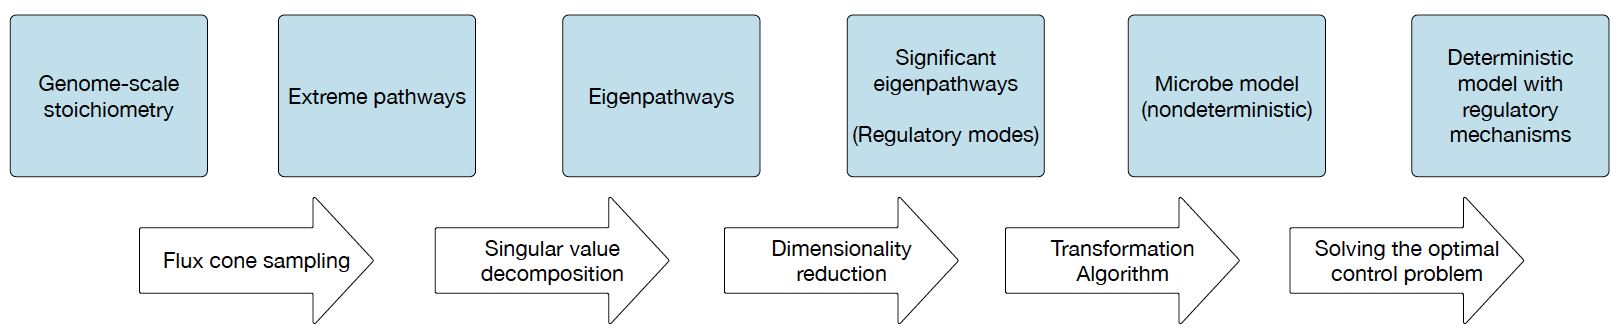
\includegraphics[width=1.1\textwidth]{figures/genome-pipeline.png}
\caption{Model generation pipeline from genome-scale stochiometry.}
\label{Organism2Automata}
\end{figure}

This pipeline can be run to completion or stopped at the stage where it generates nondeterministic models, which are particularly useful for safety analysis and full state-space exploration.

The algorithm that follows gives the detailed procedure for genome-scale model generation:

\begin{algorithm*}[H]
\SetAlgoLined
 \textbf{Input:} The trajectory $\mathbb{T} = (\mathbb{D},\overline{V} = [v_1, v_2, v_3..., v_n]) = \mathbb{D}(\overline{V})$\;
\KwResult{Hybrid automaton $\mathbb{H}(\mathbb{D},\overline{V})$ that follows trajectory $\mathbb{D}(\overline{V})$\;}

 Initialize a hybrid automaton $\mathbb{H}$ where:\\ 
 \hspace*{10mm}Continuous variables $X = \overline{C}_{ext} \cup \{ \tau \}$;\ \\
  \hspace*{10mm}Discrete locations $L = \{ l_1, l_2, ..., l_n \}$;\ \\
  \hspace*{10mm}Initial condition  $I = (l_1,[\overline{C}_{0}, 0])$;\ \\
 \hspace*{10mm}Assign the dynamics of $l_1$ as:\\ 
                        \hspace*{20mm}$\frac{d\overline{C}_{ext}}{dt} = T \cdot v_1 * Bio$\;
                        \hspace*{20mm}$\frac{d\tau}{dt} = 1$\;
 
 \For{$i = 2; i <= n$}{
    Assign the dynamics of $l_i$ as follows:\\
                        \hspace*{10mm}$\frac{d\overline{C}_{ext}}{dt} = T \cdot v_i * Bio$\;
                        \hspace*{10mm}$\frac{d\tau}{dt} = 1$\;
    
    Add a forced transition from $l_{i-1}$ to $l_i$\ with guard condition $\tau > \Delta t$ and reset $\tau = 0$;
 }
 \textbf{Return} $\mathbb{H}$;\
 \caption{Transformation of dFBA trajectory $\mathbb{D}(\overline{V})$ to hybrid automaton $\mathbb{H}(\mathbb{D},\overline{V})$}
 \label{Algo3}
\end{algorithm*}

\section{Other Convex Basis Parameterizations}

\subsection{Elementary Mode Analysis}

Alternate convex basis representations of the flux cones should also be considered as lending interperability to the model. One of the most promising of these is the set of elementary modes $M = \{ m_1, m_2, ... m_m \}$ for a given stoichiometric matrix $S$.